\documentclass[border=2pt]{standalone}

\usepackage[T1]{fontenc}
\usepackage{times}
\usepackage{graphicx}
\usepackage{xcolor}
\usepackage{booktabs}
\usepackage{array}

\begin{document}
\scriptsize
\setlength{\tabcolsep}{3pt}
\renewcommand{\arraystretch}{1.15}
\begin{tabular}{@{}c l m{6cm} c c c c@{}}
\toprule
\textbf{Canvas} & \textbf{Variant} & \textbf{Description edit} &
  \textbf{Tools} & \textbf{Think} & \textbf{Out} & \textbf{Time\,(s)} \\
\midrule
\multicolumn{7}{@{}l}{Group A. Endpoint hint on \texttt{add\_semicircle.p1/p2}.} \\
\midrule
\raisebox{-0.45\height}{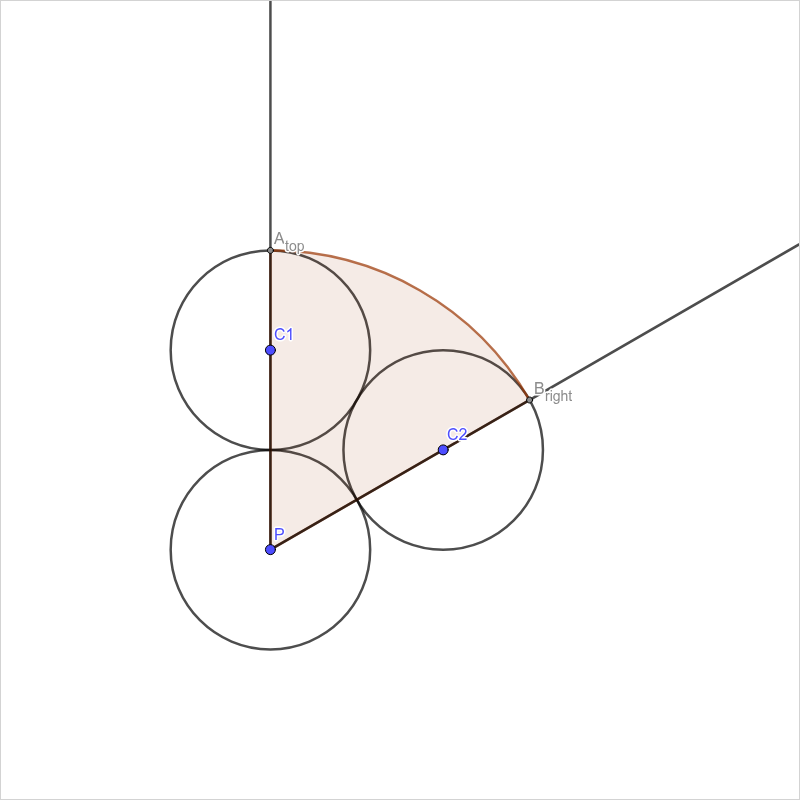
\includegraphics[width=1.4cm]{batch_v0_v9/v0_source.png}} &
  \texttt{v0\_source} & --- (unmodified ToolSpec catalog as reference) &
  13 & 11{,}097 & 1{,}001 & 75.9 \\
\raisebox{-0.45\height}{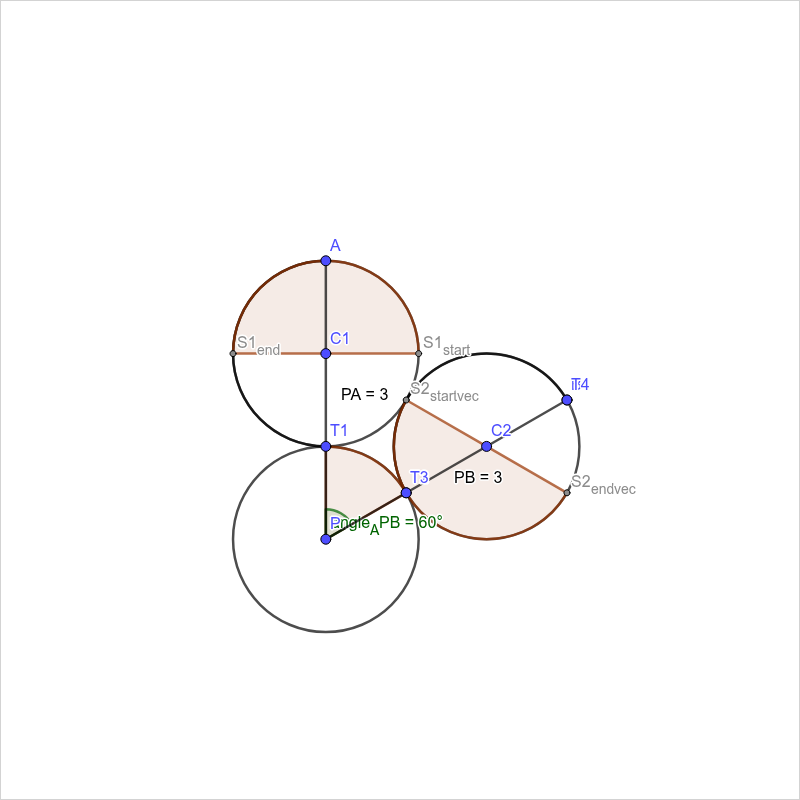
\includegraphics[width=1.4cm]{batch_v0_v9/v1_semicircle_minimal.png}} &
  \texttt{v1\_minimal} &
  \texttt{p1}: ``First endpoint of diameter \textbf{(on the boundary, not the centre)}''; same for \texttt{p2} &
  28 & 5{,}338\textsubscript{\textcolor{gray}{$-$52\%}} & 907 & 46.6 \\
\raisebox{-0.45\height}{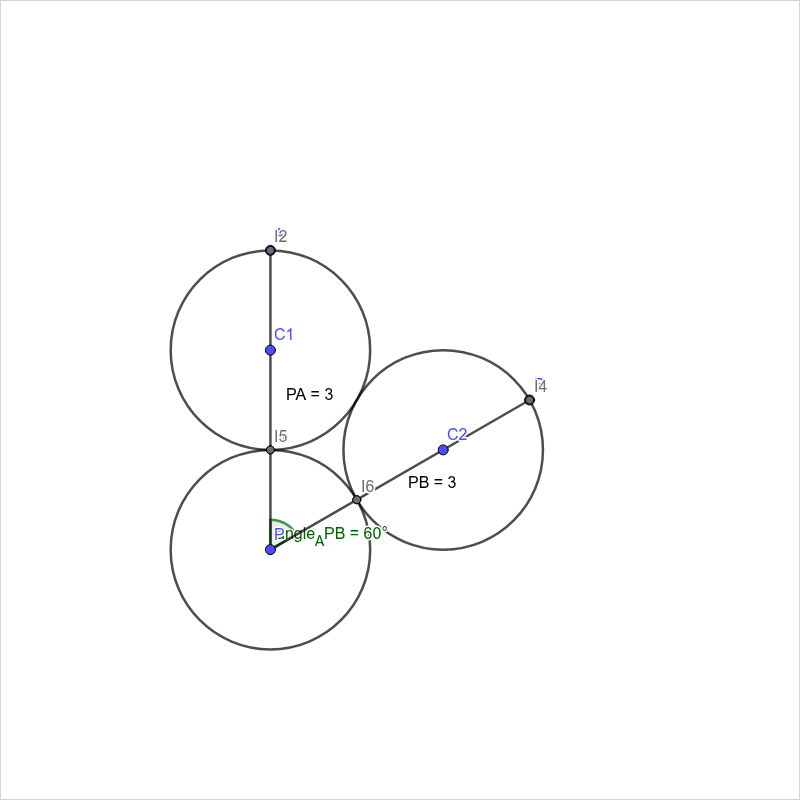
\includegraphics[width=1.4cm]{batch_v0_v9/v2_semicircle_verbose.png}} &
  \texttt{v2\_verbose} &
  \texttt{p1}: ``First endpoint of diameter\textbf{; must be a named point on the boundary, not the centre. If the endpoint is missing, create it first.}'' \par
  \texttt{p2}: ``Second\ldots\textbf{[same rule]}'' &
  17 & 7{,}252\textsubscript{\textcolor{gray}{$-$35\%}} & 1{,}150 & 52.0 \\
\midrule
\multicolumn{7}{@{}l}{Group B. CCW direction hint on \texttt{add\_arc} / \texttt{add\_sector}.} \\
\midrule
\raisebox{-0.45\height}{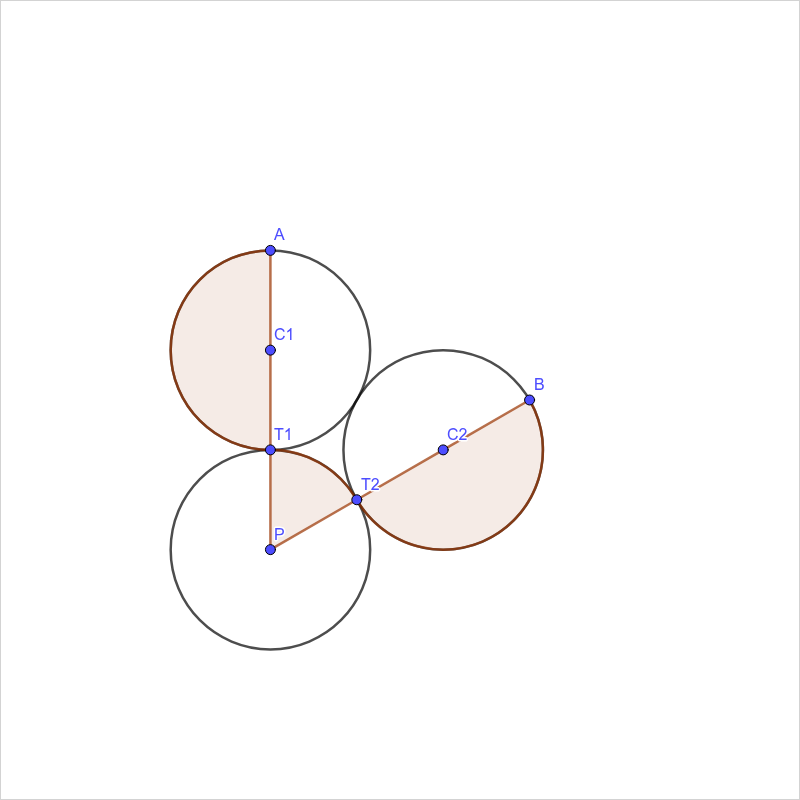
\includegraphics[width=1.4cm]{batch_v0_v9/v3_arc_short.png}} &
  \texttt{v3\_arc} &
  \texttt{add\_arc}: ``\ldots\textbf{For the shorter arc, choose start\_pt and end\_pt so the CCW sweep is the smaller sweep; otherwise swap them.}'' &
  19 & 4{,}916\textsubscript{\textcolor{gray}{$-$56\%}} & \textbf{586} & 40.2 \\
\raisebox{-0.45\height}{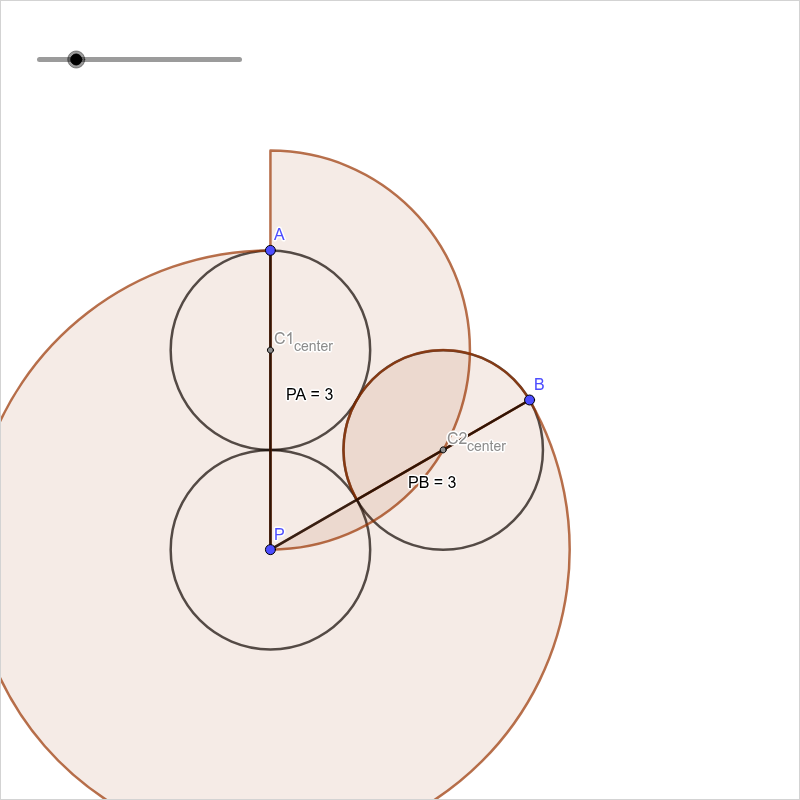
\includegraphics[width=1.4cm]{batch_v0_v9/v4_sector_short.png}} &
  \texttt{v4\_sector} &
  \texttt{add\_sector}: ``\ldots\textbf{For the smaller sector, choose start\_pt and end\_pt so the CCW sweep is the smaller sweep; otherwise swap them.}'' &
  19 & \textbf{2{,}628}\textsubscript{\textcolor{gray}{$-$76\%}} & 1{,}057 & 28.2 \\
\raisebox{-0.45\height}{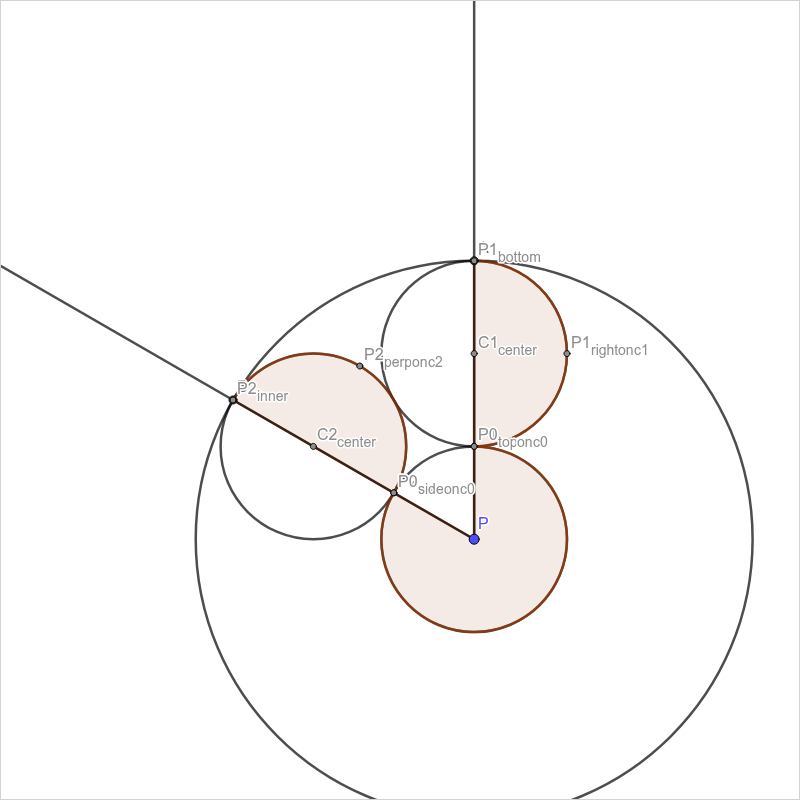
\includegraphics[width=1.4cm]{batch_v0_v9/v5_arc_sector_short.png}} &
  \texttt{v5\_both} &
  Both \texttt{add\_arc} and \texttt{add\_sector} CCW hints (= \texttt{v3} \(\cup\) \texttt{v4}) &
  26 & 4{,}295\textsubscript{\textcolor{gray}{$-$61\%}} & 1{,}480 & 37.3 \\
\midrule
\multicolumn{7}{@{}l}{Group C. Endpoint $\cup$ CCW combined.} \\
\midrule
\raisebox{-0.45\height}{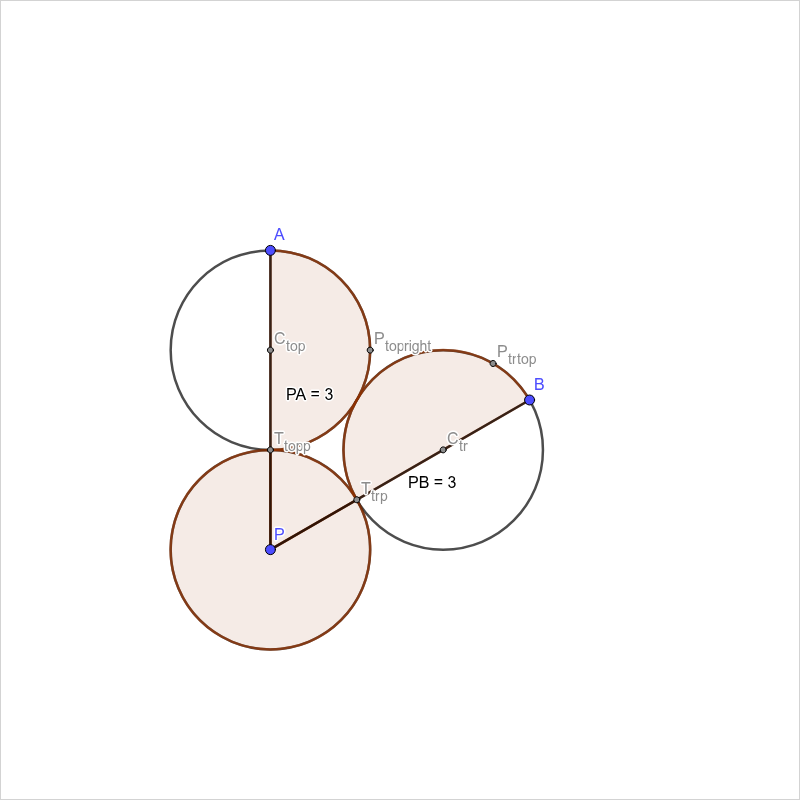
\includegraphics[width=1.4cm]{batch_v0_v9/v6_semicircle_minimal_arc_sector.png}} &
  \texttt{v6\_min+CCW} &
  \texttt{v1} $\cup$ \texttt{v3} $\cup$ \texttt{v4} (minimal endpoint + both CCW hints) &
  22 & 6{,}002\textsubscript{\textcolor{gray}{$-$46\%}} & 744 & 48.5 \\
\raisebox{-0.45\height}{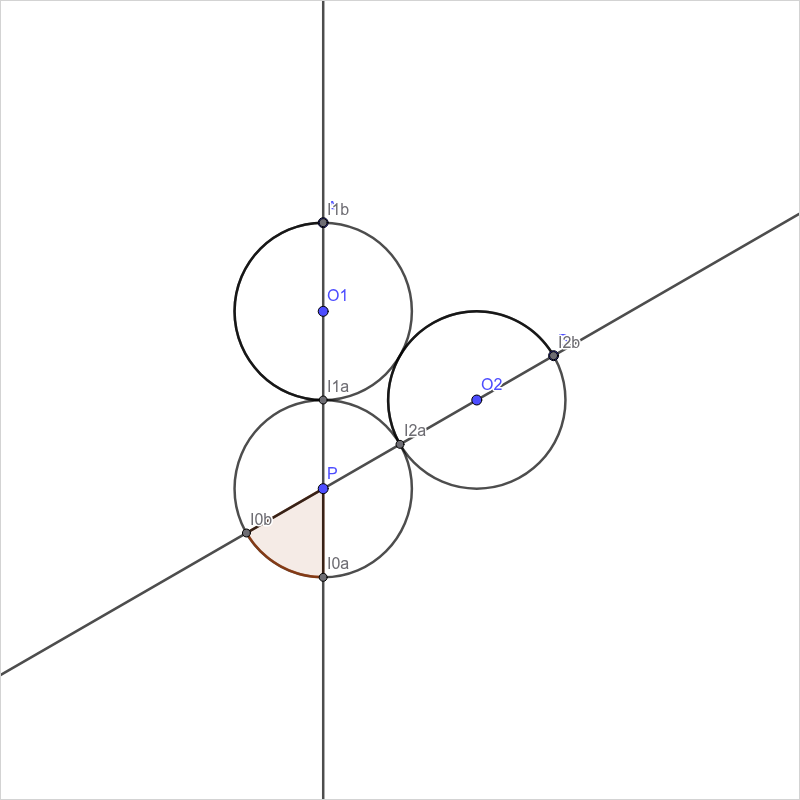
\includegraphics[width=1.4cm]{batch_v0_v9/v7_semicircle_verbose_arc_sector.png}} &
  \texttt{v7\_verb+CCW} &
  \texttt{v2} $\cup$ \texttt{v3} $\cup$ \texttt{v4} (verbose endpoint + both CCW hints) &
  23 & 3{,}182\textsubscript{\textcolor{gray}{$-$71\%}} & 738 & \textbf{28.0} \\
\midrule
\multicolumn{7}{@{}l}{Group D. Negative control (edit on a tool the trajectory never invokes).} \\
\midrule
\raisebox{-0.45\height}{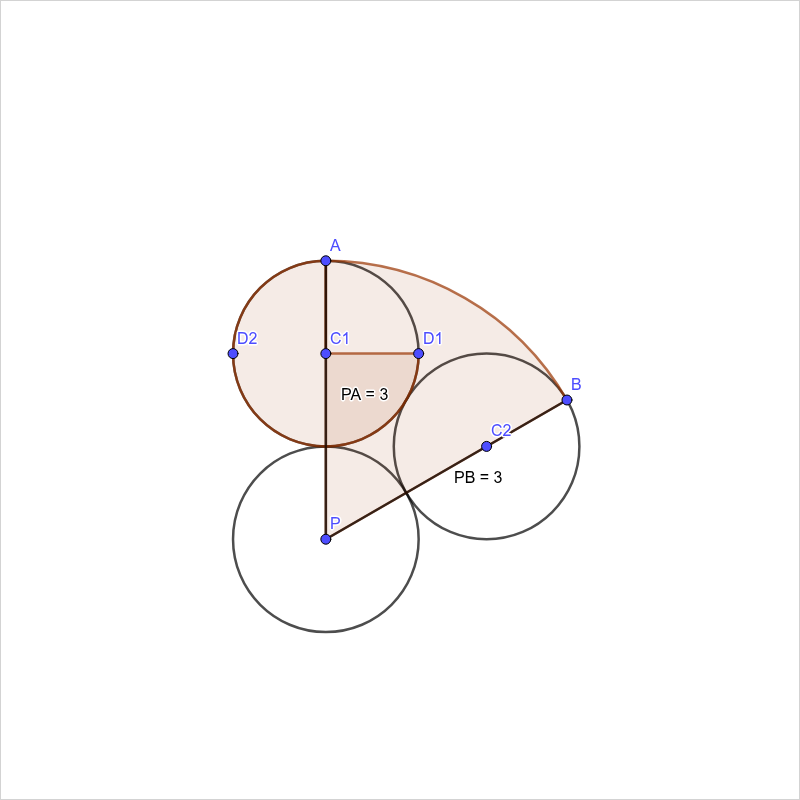
\includegraphics[width=1.4cm]{batch_v0_v9/v8_negcontrol.png}} &
  \texttt{v8\_negctrl} &
  \texttt{add\_function}: ``\ldots\textbf{Useful for plotting algebraic curves over a domain.}'' \emph{(unused on this trajectory)} &
  17 & 7{,}175\textsubscript{\textcolor{gray}{$-$35\%}} & 986 & 53.5 \\
\bottomrule
\end{tabular}
\end{document}
